
\documentclass{beamer}
\usepackage[utf8]{inputenc}

\usetheme{Madrid}
\usecolortheme{default}
\usepackage{amsmath,amssymb,amsfonts,amsthm}
\usepackage{txfonts}
\usepackage{tkz-euclide}
\usepackage{listings}
\usepackage{adjustbox}
\usepackage{array}
\usepackage{tabularx}
\usepackage{gvv}
\usepackage{lmodern}
\usepackage{circuitikz}
\usepackage{tikz}
\usepackage{graphicx}

\setbeamertemplate{page number in head/foot}[totalframenumber]

\usepackage{tcolorbox}
\tcbuselibrary{minted,breakable,xparse,skins}



\definecolor{bg}{gray}{0.95}
\DeclareTCBListing{mintedbox}{O{}m!O{}}{%
  breakable=true,
  listing engine=minted,
  listing only,
  minted language=#2,
  minted style=default,
  minted options={%
    linenos,
    gobble=0,
    breaklines=true,
    breakafter=,,
    fontsize=\small,
    numbersep=8pt,
    #1},
  boxsep=0pt,
  left skip=0pt,
  right skip=0pt,
  left=25pt,
  right=0pt,
  top=3pt,
  bottom=3pt,
  arc=5pt,
  leftrule=0pt,
  rightrule=0pt,
  bottomrule=2pt,
  toprule=2pt,
  colback=bg,
  colframe=orange!70,
  enhanced,
  overlay={%
    \begin{tcbclipinterior}
    \fill[orange!20!white] (frame.south west) rectangle ([xshift=20pt]frame.north west);
    \end{tcbclipinterior}},
  #3,
}
\lstset{
    language=C,
    basicstyle=\ttfamily\small,
    keywordstyle=\color{blue},
    stringstyle=\color{orange},
    commentstyle=\color{green!60!black},
    numbers=left,
    numberstyle=\tiny\color{gray},
    breaklines=true,
    showstringspaces=false,
}
\begin{document}

\title 
{1.6.15}
\date{August 23,2025}


\author 
{Yoshita J - EE25BTECH11065}






\frame{\titlepage}
\begin{frame}{Question}
 Find the value of m if the points $\vec(5,1)$, $\vec(-2,-3)$ and $\vec(8,2m)$ are collinear
\end{frame}



\begin{frame}{Theoretical Solution}
Let $\vec{A}(5,1)$, $\vec{B}(-2,-3)$, $\vec{C}(8,2m)$.
\\
\begin{table}[H]    
  \centering
  

  \caption{Answers}
  \label{Answers}
\end{table}
\end{frame}
\begin{frame}{Theoretical Solution}
Using the collinearity $\brak{rank}$ test, form the matrix with difference vectors:
\begin{align*}
    (\vec{B}-\vec{A} \quad \vec{C}-\vec{A}) &= \myvec{-2-5 & 8-5 \\ -3-1 & 2m-1} \\
    &= \myvec{-7 & 3 \\ -4 & 2m-1}.
\end{align*}
\end{frame}

\begin{frame}{Equation}
\textbf{The three points are collinear$\iff$this matrix has rank 1 $\brak{its\ rows\ are\ linearly\ dependent}$.\\}
\end{frame}
\begin{frame}{Theoretical Solution}
Using row reduction ,
\begin{center}
 $R_2 \leftarrow 7R_2 - 4R_1 \implies \myvec{ -7 & 3 \\ 0 & 14m-19 }.$
 \end{center}

For rank $1$, the second row must be zero:
\begin{center}
$14m - 19 = 0 \implies m = \frac{19}{14}$
\end{center}
\end{frame}


\begin{frame}[fragile]
    \frametitle{C Code - A function to find the value of m}

    \begin{lstlisting}
#include <stdio.h>
float find_collinear_m(float Ax, float Ay, float Bx, float By, float Cx, float coeff_m) {
    float numerator = (By - Ay) * (Cx - Ax) + Ay * (Bx - Ax);
    float denominator = coeff_m * (Bx - Ax);
    if (denominator == 0) {  
        return 0; 
    }
    return numerator / denominator;
}

    \end{lstlisting}
\end{frame}

\begin{frame}[fragile]
    \frametitle{Python Code}
    \begin{lstlisting}
import numpy as np
import matplotlib.pyplot as plt
import ctypes
import os

try:
    c_lib = ctypes.CDLL('./code.so')
except OSError:
    print("Error: 'code.so' not found.")
    print("Please ensure you have a 'code.c' file with the find_collinear_m function")
    print("and that you have a C compiler (like gcc) installed to compile it.")
    exit()


    \end{lstlisting}
\end{frame}

\begin{frame}[fragile]
    \frametitle{Python Code}
    \begin{lstlisting}
c_lib.find_collinear_m.argtypes = [
    ctypes.c_float, ctypes.c_float, # Ax, Ay
    ctypes.c_float, ctypes.c_float, # Bx, By
    ctypes.c_float, ctypes.c_float  # Cx, coeff_m
]

c_lib.find_collinear_m.restype = ctypes.c_float


A = np.array([5.0, 1.0])
B = np.array([-2.0, -3.0])
Cx = 8.0
coeff_m = 2.0 # The y-coordinate of C is 2*m


    \end{lstlisting}
\end{frame}

\begin{frame}[fragile]
    \frametitle{Python Code}
    \begin{lstlisting}
m_value = c_lib.find_collinear_m(
    ctypes.c_float(A[0]),     # Ax
    ctypes.c_float(A[1]),     # Ay
    ctypes.c_float(B[0]),     # Bx
    ctypes.c_float(B[1]),     # By
    ctypes.c_float(Cx),       # Cx
    ctypes.c_float(coeff_m)   # coeff_m
)

C = np.array([Cx, coeff_m * m_value])

print(f"The C function calculated m = {m_value:.4f}")
print(f"This corresponds to point C being at ({C[0]:.2f}, {C[1]:.2f})")
print("The exact value of m is 19/14.")
    \end{lstlisting}
\end{frame}

\begin{frame}[fragile]
    \frametitle{Python Code}
    \begin{lstlisting}
slope = (B[1] - A[1]) / (B[0] - A[0])
intercept = A[1] - slope * A[0]

x_min = min(A[0], B[0], C[0]) - 2
x_max = max(A[0], B[0], C[0]) + 2
x_line = np.linspace(x_min, x_max, 100)
y_line = slope * x_line + intercept

plt.plot(x_line, y_line, label=f'Line through A, B, and C (m={m_value:.2f})', color='blue')

all_points = np.vstack((A, B, C)).T
plt.scatter(all_points[0, :], all_points[1, :], color='red', zorder=5)

    \end{lstlisting}
\end{frame}
\begin{frame}[fragile]
    \frametitle{Python Code}
    \begin{lstlisting}
point_labels = [f'A ({A[0]},{A[1]})', f'B ({B[0]},{B[1]})', f'C ({C[0]:.1f},{C[1]:.2f})']
for i, txt in enumerate(point_labels):
    plt.annotate(txt,
                 (all_points[0, i], all_points[1, i]),
                 textcoords="offset points",
                 xytext=(10, 5),
                 ha='center')


plt.xlabel('$x$')
plt.ylabel('$y$')
plt.title('Visualization of Collinear Points')
plt.legend(loc='best')
plt.grid(True)
plt.axis('equal')

plt.savefig('..figs\collinear_points.png')

plt.show()
    \end{lstlisting}
\end{frame}

\begin{frame}{Plot}
    \centering
    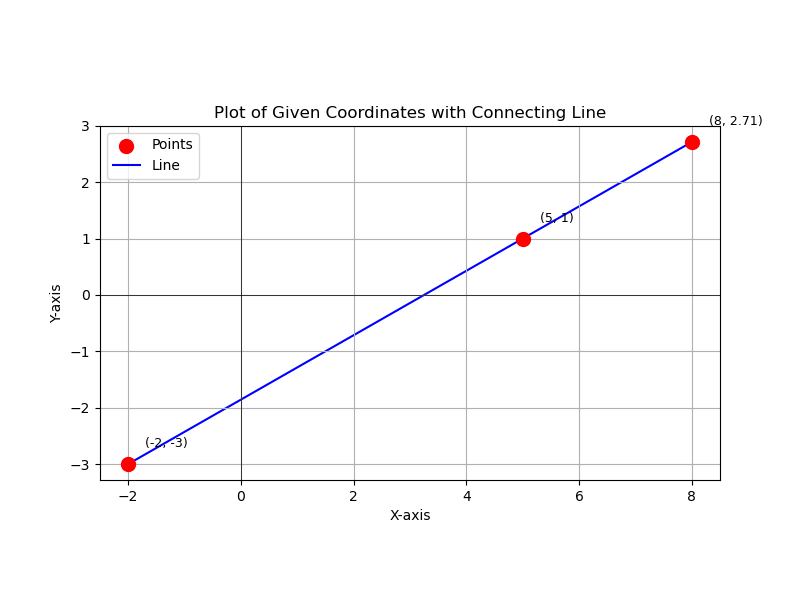
\includegraphics[width=\columnwidth, height=0.8\textheight, keepaspectratio]{figs/fig.png}     
\end{frame}


\end{document}
